% future.tex -- three mutually reinforcing future directions.

\documentclass[tikz,border=3pt]{standalone}
\usepackage[dvipsnames]{xcolor}
\usetikzlibrary{arrows.meta,positioning}

\newcommand{\PredRW}{\mathsf{PredRW}}
\newcommand{\PredRWCAV}{\mathsf{PredRW}^{-}}
\newcommand{\PredRWarXiv}{\mathsf{PredRW}^{+}}

\begin{document}
  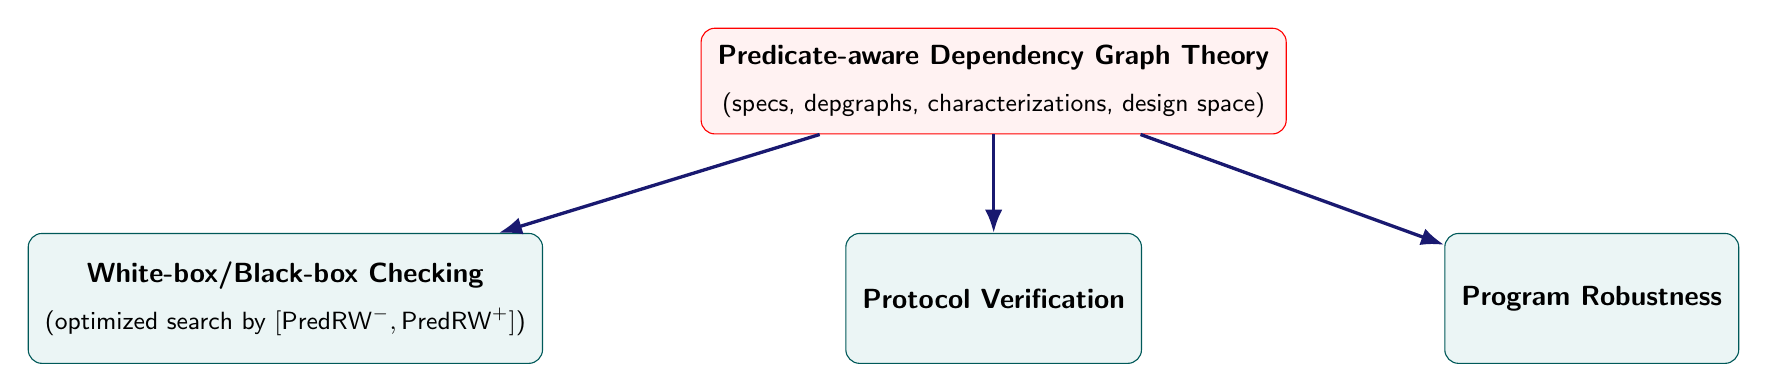
\begin{tikzpicture}[
    >=Latex,font=\sffamily,
    core/.style={draw=red,rounded corners=5pt,fill=red!5,
      align=center,minimum width=3.8cm,minimum height=1.2cm,inner sep=6pt},
    dir/.style={draw=teal!70!black,rounded corners=5pt,fill=teal!8,
      align=center,minimum width=3.45cm,minimum height=1.65cm,inner sep=6pt}]
    \node[core] (core) {\textbf{Predicate-aware Dependency Graph Theory}
      \\[5pt]\small (specs, depgraphs, characterizations, design space)};
    \node[dir,below left=1.25cm and 2.0cm of core] (checking)
      {\textbf{White-box/Black-box Checking}
      \\[5pt] \small (optimized search
        by $[\PredRWCAV, \PredRWarXiv]$)};
    \node[dir,below=1.25cm of core] (rob)
      {\textbf{Protocol Verification}};
    \node[dir,below right=1.25cm and 2.0cm of core] (db)
      {\textbf{Program Robustness}};
    \draw[-Latex,very thick,MidnightBlue] (core) -- (checking);
    \draw[-Latex,very thick,MidnightBlue] (core) -- (rob);
    \draw[-Latex,very thick,MidnightBlue] (core) -- (db);
  \end{tikzpicture}
\end{document}